


\pgfplotsset{compat=1.18}

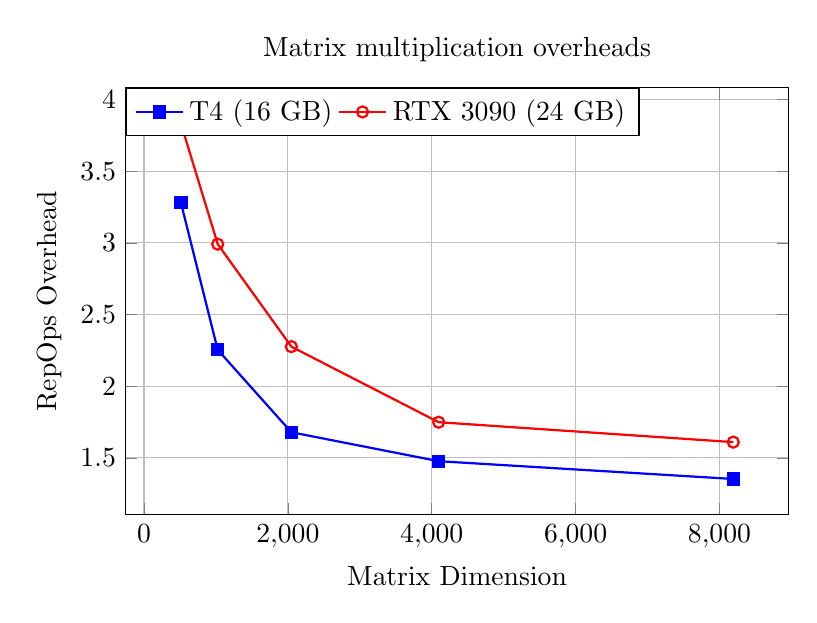
\begin{tikzpicture}
\begin{axis}[
    width=10cm, %
    height=7cm, %
    xlabel={Matrix Dimension}, %
    ylabel={RepOps Overhead}, %
    grid=both, %
    legend style={at={(0,1)}, anchor=north west, legend columns=2},
    title={Matrix multiplication overheads},
    extra y ticks={0},
extra y tick style={
  grid=major,
  major grid style={dashed,line width=0.5pt, black}
}
]

\addplot[
    color=blue, 
    mark=square*, 
    thick
]
coordinates {
    (512, 3.281)
    (1024, 2.254)
    (2048, 1.679)
    (4096, 1.477)
    (8192, 1.353)
};

 

\addplot[
    color=red, 
    mark=o, 
    thick
] 
coordinates {
    (512, 3.833)
    (1024, 2.991)
    (2048, 2.276)
    (4096, 1.749)
    (8192, 1.610)
};


\legend{T4 (16 GB), RTX 3090 (24 GB)}
\end{axis}
\end{tikzpicture}



